\documentclass[oneside, french, a4paper, 12pt, reqno]{book}
\usepackage[utf8]{inputenc}
\usepackage[T1]{fontenc}
\usepackage{lmodern}
\usepackage[main=french]{babel}
\usepackage[left=2.5cm,right=2.5cm,top=2.5cm,bottom=2.5cm,headheight=15pt]{geometry}

% Packages essentiels pour mise en forme
\usepackage{xcolor}
\usepackage{tikz}
\usepackage{tcolorbox}
\usepackage[explicit]{titlesec}
\usepackage{fancyhdr}
\usepackage{caption}
\usepackage{subcaption}
\usepackage{setspace}
\usepackage{enumitem}
\usepackage{array,ragged2e}
\usepackage{multirow}
\usepackage{booktabs}
\usepackage{longtable}
\usepackage{float}
\usepackage{wrapfig}
\usepackage{chngcntr}
\usepackage[bottom]{footmisc}
\usepackage{minitoc}
\usepackage{graphicx}
\usepackage{needspace}

% Packages pour math et code
\usepackage{amsmath,amssymb,amsfonts}
\usepackage{extarrows}
\usepackage{siunitx}
\usepackage{listings}
\usepackage{algorithm}
\usepackage{algpseudocode}  % Remplace algorithmic (déprécié)
\usepackage{pgfplots}

% Autres packages utiles
\usepackage{xspace}
\usepackage[normalem]{ulem}
\usepackage{soul}
\usepackage{scrextend}
\usepackage{colortbl}
\usepackage{wasysym}
\usepackage{adjustbox}
\usepackage{changepage}
\usepackage{hhline}
\usepackage{multicol}
\usepackage{makecell}
\usepackage{tabto}
\usepackage{textcomp}
\usepackage{lipsum}
\usepackage{flowchart}
\usepackage[toc,page]{appendix}

% Package important à charger avant hyperref
\usepackage[nottoc]{tocbibind}

% Packages pour la typographie française
\usepackage{csquotes}  % Pour les guillemets français
\usepackage[autolanguage]{numprint}  % Formatage des nombres en français
\usepackage{microtype}  % Amélioration de la typographie

% Hyperliens (TOUJOURS charger en dernier)
\usepackage[hidelinks]{hyperref}

% Configuration PDF et métadonnées
\hypersetup{
    pdftitle={Système de Détection d'Anomalies pour Moteurs Industriels basé sur l'Intelligence Artificielle Embarquée},
    pdfauthor={Ahmed Abdellahi Abdat},
    pdfsubject={Projet de Fin d'Études - Master EEA - FSB},
    pdfkeywords={TinyML, Maintenance prédictive, ESP32, Détection d'anomalies, K-means}
}

% Configuration TikZ et PGFPlots
\usetikzlibrary{shapes.symbols,shapes.geometric,shadows,arrows.meta,calc,positioning}
\tikzset{>={Latex[width=1.5mm,length=2mm]}}
\pgfplotsset{width=10cm,compat=1.9}

% Définition des couleurs
\definecolor{chapterColor}{RGB}{0,0,0}     % Noir (cohérence académique)
\definecolor{sectionColor}{RGB}{0,0,0}   % Noir (standard académique)
\definecolor{tableRow1}{RGB}{210,234,241}     % Gris-bleu clair
\definecolor{gray75}{gray}{0.75}
\definecolor{Gris1}{RGB}{116,134,170}
\definecolor{Gris2}{RGB}{249,249,249}
\definecolor{mygreen}{RGB}{28,172,0}
\definecolor{mylilas}{RGB}{170,55,241}
\definecolor{MyBlue}{HTML}{4c72b0}
\definecolor{MyGreen}{HTML}{55a868}
\definecolor{MyOrange}{HTML}{dd8452}
\definecolor{MyRed}{HTML}{c44e52}

%%%%%%%%%%%%%%%%%%%%%%%%%%%%%%%%%%%%%%%%%%%%%%%%%%%%%%%%%%%
% STYLE DES CHAPITRES - PLEINE PAGE
%%%%%%%%%%%%%%%%%%%%%%%%%%%%%%%%%%%%%%%%%%%%%%%%%%%%%%%%%%%

% Style pour les chapitres numérotés (page complète)
\titleformat{\chapter}[display]%
  {\normalfont\huge\bfseries}%
  {}%
  {0pt}%
  {\thispagestyle{plain}\vspace*{\fill}%
   \begin{center}%
     % Ligne supérieure décorative
     \textcolor{chapterColor}{\rule{0.5\textwidth}{2pt}}\\[2cm]%
     % Mot "CHAPITRE"
     {\Large\scshape\color{gray75}CHAPITRE}\\[\baselineskip]%
     % Grande boîte avec le numéro
     \colorbox{chapterColor}{%
       \parbox[c][3cm][c]{3cm}{%
         \centering\textcolor{white}{\fontsize{60}{60}\selectfont\bfseries\thechapter}%
       }%
     }\\[2cm]%
     % Titre du chapitre
     {\Huge\bfseries\color{chapterColor}#1}\\[2cm]%
     % Ligne inférieure décorative
     \textcolor{chapterColor}{\rule{0.5\textwidth}{2pt}}%
   \end{center}%
   \vspace*{\fill}\newpage%
  }

% Chapitres non numérotés (style ENETCOM avec boîte colorée à gauche)
\newlength\BoxWd
\setlength\BoxWd{10mm}
\titleformat{name=\chapter, numberless}[display]%
  {\fontsize{26}{6}\bfseries\selectfont}%
  {%
    {\hspace*{-1.5mm}\normalfont\fontsize{14}{6}\selectfont{~}}\\%
    \colorbox{chapterColor}{%
      \parbox[c][20mm][t]{\BoxWd}{%
        \vspace{2.5mm}\centering\textcolor{white}{~}%
      }%
    }%
  }%
  {-10mm}%
  {%
    \vspace{-5mm}\hspace*{15mm}\titlerule[2pt]\\\\\hspace*{15mm}#1%
  }

% Espacement des chapitres
\titlespacing*{\chapter}{0pt}{0pt}{0pt}
\titlespacing*{name=\chapter,numberless}{0pt}{50pt}{30pt}

% Espacement des sections (conforme aux normes académiques)
% Format: \titlespacing{command}{left}{before}{after}
\titlespacing*{\section}{0pt}{3.5ex plus 1ex minus .2ex}{2.3ex plus .2ex}
\titlespacing*{\subsection}{0pt}{3.25ex plus 1ex minus .2ex}{1.5ex plus .2ex}
\titlespacing*{\subsubsection}{0pt}{3.25ex plus 1ex minus .2ex}{1.5ex plus .2ex}

%%%%%%%%%%%%%%%%%%%%%%%%%%%%%%%%%%%%%%%%%%%%%%%%%%%%%%%%%%%
% STYLE DES SECTIONS ET SOUS-SECTIONS
%%%%%%%%%%%%%%%%%%%%%%%%%%%%%%%%%%%%%%%%%%%%%%%%%%%%%%%%%%%
\titleformat{\section}[block]%
  {\Large\bfseries\color{sectionColor}}{\thesection}%
  {1em}{\Large{#1}}  % Utilise em au lieu de pt, supprime le bfseries redondant
  
\titleformat{\subsection}[block]%
  {\large\bfseries\color{sectionColor}}{\thesubsection}%
  {0.8em}{\large{#1}}

\titleformat{\subsubsection}[block]%
  {\normalsize\bfseries\color{sectionColor}}{\thesubsubsection}%
  {0.6em}{\normalsize{#1}}

%%%%%%%%%%%%%%%%%%%%%%%%%%%%%%%%%%%%%%%%%%%%%%%%%%%%%%%%%%%
% Configuration du code source
%%%%%%%%%%%%%%%%%%%%%%%%%%%%%%%%%%%%%%%%%%%%%%%%%%%%%%%%%%%
\lstdefinestyle{mystyle}{
    backgroundcolor=\color{Gris2},
    commentstyle=\color{mygreen},
    keywordstyle=\color{blue},
    numberstyle=\tiny\color{gray},
    stringstyle=\color{mylilas},
    basicstyle=\ttfamily\footnotesize,
    breakatwhitespace=false,
    breaklines=true,
    captionpos=b,
    keepspaces=true,
    numbers=left,
    numbersep=5pt,
    showspaces=false,
    showstringspaces=false,
    showtabs=false,
    tabsize=2,
    frame=single,
    rulecolor=\color{gray75}
}
\lstset{style=mystyle}

%%%%%%%%%%%%%%%%%%%%%%%%%%%%%%%%%%%%%%%%%%%%%%%%%%%%%%%%%%%
% CONFIGURATION DES LÉGENDES
%%%%%%%%%%%%%%%%%%%%%%%%%%%%%%%%%%%%%%%%%%%%%%%%%%%%%%%%%%%
\captionsetup{
  labelfont=bf,
  font={singlespacing,small},
  justification=centering,
  textfont=it
}

% Configuration des marges et espacements
\setcounter{tocdepth}{3}
\setcounter{secnumdepth}{3}
\setlistdepth{9}
\counterwithout{footnote}{chapter}

% Configuration des listes
\renewlist{enumerate}{enumerate}{9}
\setlist[enumerate,1]{label=\arabic*.}
\setlist[enumerate,2]{label=\alph).}
\renewlist{itemize}{itemize}{9}
\setlist[itemize,1]{label=\textbullet}
\setlist[itemize,2]{label=\textendash}
\setlist[itemize,3]{label=$\ast$}

% Configuration de l'espacement des paragraphes
\setlength{\parskip}{1.5ex plus 0.5ex minus 0.2ex}  % Espace flexible entre paragraphes (5-7mm)
\setlength{\parindent}{0pt}  % Pas d'indentation (standard français moderne)
\frenchspacing  % Espacement français correct
\raggedbottom  % Évite l'étirement vertical des pages
\renewcommand\bibname{Bibliographie}
\newcommand{\HRule}[1][\linewidth]{\rule{#1}{0.5mm}}
\renewcommand{\arraystretch}{1.3}

% Éviter les césures
\hyphenpenalty=10000
\exhyphenpenalty=10000

% Configuration minitoc
\dominitoc
\mtcsettitle{minitoc}{Sommaire}
\mtcsetdepth{minitoc}{2}

%%%%%%%%%%%%%%%%%%%%%%%%%%%%%%%%%%%%%%%%%%%%%%%%%%%%%%%%%%%
% EN-TÊTES ET PIEDS DE PAGE STYLE PROFESSIONNEL
%%%%%%%%%%%%%%%%%%%%%%%%%%%%%%%%%%%%%%%%%%%%%%%%%%%%%%%%%%%
\fancypagestyle{pfeStyle}{
  \renewcommand{\headrulewidth}{0.5pt}
  \renewcommand{\footrulewidth}{0.5pt}
  \fancyhf{}
  \fancyhead[C]{\fontsize{11}{11}\selectfont\nouppercase{\leftmark}}
  \fancyfoot[L]{\fontsize{10}{10}\selectfont FSB - Master EEA}
  \fancyfoot[C]{\fontsize{10}{10}\selectfont Page \thepage}
  \fancyfoot[R]{\fontsize{10}{10}\selectfont 2024-2025}
}

\fancypagestyle{plain}{
  \renewcommand{\headrulewidth}{0pt}
  \renewcommand{\footrulewidth}{0.5pt}
  \fancyhf{}
  \fancyfoot[L]{\fontsize{10}{10}\selectfont FSB - Master EEA}
  \fancyfoot[C]{\fontsize{10}{10}\selectfont Page \thepage}
  \fancyfoot[R]{\fontsize{10}{10}\selectfont 2024-2025}
}

% Configuration pour n'afficher que les chapitres dans les en-têtes (sans les sections)
\renewcommand{\chaptermark}[1]{\markboth{\chaptername\ \thechapter.\ #1}{}}
\renewcommand{\sectionmark}[1]{} % Désactiver les sections dans les en-têtes

% Commande pour page blanche
\newcommand\blankpage{%
    \null
    \thispagestyle{empty}%
    \addtocounter{page}{-1}%
    \newpage}

%%%%%%%%%%%%%%%%%%%%%%%%%%%%%%%%%%%%%%%%%%%%%%%%%%%%%%%%%%%
% DÉBUT DU DOCUMENT
%%%%%%%%%%%%%%%%%%%%%%%%%%%%%%%%%%%%%%%%%%%%%%%%%%%%%%%%%%%
\begin{document}

% Configuration du style de page
\pagestyle{pfeStyle}
\frontmatter  % Numérotation romaine pour les pages liminaires

%%%%%%%%%%%%%%%%%%%%%%%%%%%%%%%%%%%%%%%%%%%%%%%%%%%%%%%%%%%
% PAGE DE GARDE
%%%%%%%%%%%%%%%%%%%%%%%%%%%%%%%%%%%%%%%%%%%%%%%%%%%%%%%%%%%
\begin{titlepage}
    \thispagestyle{empty}
    \begin{center}
        \vspace*{-2cm}
        
        % En-tête institutionnel
        \textsc{\Large Université de Sfax}\\[0.5cm]
        \textsc{\Large Faculté des Sciences de Sfax}\\[0.5cm]
        \textsc{Département de Physique}\\[1.5cm]
        
        % Encadré du titre principal
        \HRule[0.8\textwidth]\\[0.4cm]
        {\huge\bfseries PROJET DE FIN D'ÉTUDES}\\[0.2cm]
        \HRule[0.8\textwidth]\\[1.5cm]
        
        % Titre du projet dans un cadre coloré
        \begin{tcolorbox}[
            colback=Gris2,
            colframe=chapterColor,
            boxrule=2pt,
            arc=0mm,
            width=0.9\textwidth,
            center
        ]
            \centering
            \Large\bfseries Système de Détection d'Anomalies pour\\
            Moteurs Industriels basé sur\\
            l'Intelligence Artificielle Embarquée\\[0.5cm]
            \large Application du TinyML pour la Maintenance Prédictive
        \end{tcolorbox}
        
        \vspace{1.5cm}
        
        % Informations sur l'étudiant et l'encadrant
        \begin{minipage}{0.45\textwidth}
            \begin{flushleft}
                \large
                \textbf{Présenté par :}\\
                Ahmed Abdellahi ABDAT\\[0.5cm]
                \textbf{Encadré par :}\\
                Dr. Khalil JOUILI
            \end{flushleft}
        \end{minipage}
        \hfill
        \begin{minipage}{0.45\textwidth}
            \begin{flushright}
                \large
                \textbf{Formation :}\\
                Master Électronique,\\
                Énergie Électrique et Automatique\\[0.5cm]
                \textbf{Année universitaire :}\\
                2024-2025
            \end{flushright}
        \end{minipage}
        
        \vfill
        
        % Cadre pour le jury
        \begin{tcolorbox}[
            colback=white,
            colframe=gray75,
            boxrule=1pt,
            arc=2mm,
            width=0.8\textwidth,
            center
        ]
            \centering\large\textbf{Jury de Soutenance}\\[0.5cm]
            \begin{tabular}{ll}
                \textbf{Président :} & Pr. [À définir] \\
                \textbf{Rapporteur :} & Dr. Khalil JOUILI \\
                \textbf{Examinateur :} & Dr. [À définir] \\
            \end{tabular}
        \end{tcolorbox}
        
        \vspace{1cm}
        Date de soutenance : \_\_\_\_\_\_\_\_\_\_\_\_
    \end{center}
\end{titlepage}

%%%%%%%%%%%%%%%%%%%%%%%%%%%%%%%%%%%%%%%%%%%%%%%%%%%%%%%%%%%
% REMERCIEMENTS avec DÉDICACE intégrée
%%%%%%%%%%%%%%%%%%%%%%%%%%%%%%%%%%%%%%%%%%%%%%%%%%%%%%%%%%%
\chapter*{REMERCIEMENTS}
\addcontentsline{toc}{chapter}{Remerciements}
\thispagestyle{plain}

\vspace{0.5cm}
\begin{center}
    \Large\itshape
    À mes parents, pour leur amour et leur soutien inconditionnel\\[0.5cm]
    À mes frères et sœurs, pour leurs encouragements constants
\end{center}
\vspace{1cm}

\begin{large}
Nos remerciements vont tout d'abord à \textbf{Dieu Tout-Puissant} pour la volonté, la santé et la patience qu'Il nous a accordées durant toutes ces années.

Nous exprimons notre profonde gratitude à nos \textbf{parents}, ainsi qu'à nos \textbf{frères et sœurs}, qui nous ont soutenus par leurs encouragements tout au long de nos études.

Nous adressons également nos plus sincères remerciements à \textbf{Dr. Khalil Jouili}, pour son encadrement, ses conseils méthodologiques et sa disponibilité tout au long de ce projet.

Enfin, nous remercions toute personne, de près ou de loin, qui a contribué à rendre ce travail réalisable et présentable.
\end{large}

%%%%%%%%%%%%%%%%%%%%%%%%%%%%%%%%%%%%%%%%%%%%%%%%%%%%%%%%%%%
% RÉSUMÉS
%%%%%%%%%%%%%%%%%%%%%%%%%%%%%%%%%%%%%%%%%%%%%%%%%%%%%%%%%%%
\chapter*{RÉSUMÉ}
\addcontentsline{toc}{chapter}{Résumé}
\thispagestyle{plain}

\begin{spacing}{1.3}
Ce projet présente le développement d'un système de détection d'anomalies pour moteurs asynchrones triphasés basé sur l'intelligence artificielle embarquée (TinyML). L'approche proposée explore le potentiel du TinyML pour rendre la maintenance prédictive plus accessible aux PME industrielles, utilisant l'apprentissage non-supervisé (K-means) nécessitant uniquement des données de fonctionnement normal. Le prototype développé, d'un coût inférieur à 50€, vise une détection en temps réel avec une latence d'inférence inférieure à 10ms et une autonomie totale sans dépendance cloud. Les tests réalisés sur un moteur asynchrone triphasé (0,37 kW) au laboratoire universitaire FSB montrent une précision supérieure à 90\% dans la détection d'anomalies vibratoires simulées (résultats détaillés au Chapitre 3). Ce travail de recherche explore la faisabilité technique d'une approche TinyML pour la maintenance prédictive, une validation en conditions industrielles réelles étant nécessaire pour confirmer son applicabilité pratique.\\[0.5cm]
\end{spacing}

\vspace{0.5cm}
\noindent\textbf{Mots-clés :} TinyML, Maintenance prédictive, Microcontrôleur embarqué, Détection d'anomalies, K-means, Analyse vibratoire, Industry 4.0, Edge Computing

\chapter*{ABSTRACT}
\addcontentsline{toc}{chapter}{Abstract}
\thispagestyle{plain}

\begin{spacing}{1.3}
This project presents the development of an anomaly detection system for three-phase asynchronous motors based on embedded artificial intelligence (TinyML). The proposed approach explores the potential of TinyML to make predictive maintenance more accessible to industrial SMEs, employing unsupervised learning (K-means) requiring only normal operating data. The developed prototype, costing less than €50, targets real-time detection with inference latency below 10ms and complete autonomy without cloud dependency. Tests conducted at the FSB university laboratory on a three-phase asynchronous motor (0.37 kW) show accuracy exceeding 90\% in detecting simulated vibration anomalies (detailed results in Chapter 3). This research work explores the technical feasibility of a TinyML approach for predictive maintenance, with validation under real industrial conditions necessary to confirm its practical applicability.\\[0.5cm]
\end{spacing}

\vspace{0.5cm}
\noindent\textbf{Keywords:} TinyML, Predictive maintenance, Embedded microcontroller, Anomaly detection, K-means, Vibration analysis, Industry 4.0, Edge Computing

%%%%%%%%%%%%%%%%%%%%%%%%%%%%%%%%%%%%%%%%%%%%%%%%%%%%%%%%%%%
% TABLE DES MATIÈRES
%%%%%%%%%%%%%%%%%%%%%%%%%%%%%%%%%%%%%%%%%%%%%%%%%%%%%%%%%%%
\cleardoublepage
\renewcommand*\contentsname{TABLE DES MATIÈRES}
\addtocontents{toc}{\protect\thispagestyle{plain}}
\begin{spacing}{1}
    \tableofcontents
\end{spacing}

% Liste des tableaux
\cleardoublepage
\renewcommand{\listtablename}{LISTE DES TABLEAUX}
\addtocontents{lot}{\protect\thispagestyle{plain}}
\listoftables

% Liste des figures
\cleardoublepage
\renewcommand{\listfigurename}{LISTE DES FIGURES}
\addtocontents{lof}{\protect\thispagestyle{plain}}
\listoffigures

%%%%%%%%%%%%%%%%%%%%%%%%%%%%%%%%%%%%%%%%%%%%%%%%%%%%%%%%%%%
% LISTE DES SYMBOLES
%%%%%%%%%%%%%%%%%%%%%%%%%%%%%%%%%%%%%%%%%%%%%%%%%%%%%%%%%%%
\chapter*{LISTE DES SYMBOLES}
\addcontentsline{toc}{chapter}{Liste des symboles}
\thispagestyle{plain}

%%%%%%%%%%%%%%%%%%%%%%%%%%%%%%%%%%%%%%%%%%%%%%%%%%%%%%%%%%%
% INTRODUCTION GÉNÉRALE
%%%%%%%%%%%%%%%%%%%%%%%%%%%%%%%%%%%%%%%%%%%%%%%%%%%%%%%%%%%
\cleardoublepage
\mainmatter  % Passage à la numérotation arabe
\pagenumbering{arabic}  % Explicitly start Arabic numbering
\setcounter{page}{1}    % Start from page 1

\chapter*{Introduction Générale}
\addcontentsline{toc}{chapter}{Introduction Générale}
\thispagestyle{plain}  % Show page number at bottom center

Dans le contexte de l'Industrie 4.0, la maintenance prédictive s'affirme comme un levier essentiel pour améliorer la disponibilité des équipements et réduire les arrêts non planifiés. Elle prolonge la maintenance conditionnelle en exploitant l'analyse des données de fonctionnement — notamment les vibrations — et des méthodes d'intelligence artificielle pour détecter précocement les comportements anormaux.

Toutefois, le déploiement de solutions complètes reste difficile pour de nombreuses entreprises en raison des coûts, de la complexité d'intégration et de la dépendance à des infrastructures réseau.

Dans ce cadre, le paradigme TinyML — exécuter des modèles d'IA directement sur des microcontrôleurs — offre une alternative intéressante pour analyser au plus près de la machine, avec une faible latence, une meilleure confidentialité et des coûts contenus.

Ce mémoire présente une étude sur le développement d'un système de détection d'anomalies pour moteurs industriels basé sur TinyML, explorant le potentiel de cette technologie pour rendre la maintenance prédictive plus accessible aux petites et moyennes entreprises (PME) industrielles. Notre étude explore l'utilisation d'algorithmes d'apprentissage non-supervisé sur microcontrôleur embarqué. La validation expérimentale, réalisée en laboratoire universitaire, permet d'évaluer la faisabilité technique de cette approche.

\textbf{Note méthodologique :} Ce travail se concentre sur la \textit{faisabilité technique} d'une implémentation TinyML pour la détection d'anomalies vibratoires. Les estimations économiques citées visent à contextualiser l'enjeu stratégique, mais ne constituent pas l'objet principal de validation de ce PFE. Une évaluation économique complète (calcul de ROI, analyse coût-bénéfice sur équipements réels) nécessiterait un déploiement industriel à long terme dépassant le cadre d'un projet de fin d'études.

Le présent document est structuré comme suit :

Le \textbf{Chapitre 1} présente l'état de l'art, établissant les bases théoriques nécessaires : l'évolution de la maintenance industrielle, les concepts fondamentaux de l'analyse vibratoire et du TinyML, ainsi qu'une revue critique de la littérature récente pour identifier les lacunes et positionner notre contribution.

Les chapitres suivants, en cours de rédaction, détailleront la conception du système, sa réalisation pratique et les résultats expérimentaux obtenus.

%%%%%%%%%%%%%%%%%%%%%%%%%%%%%%%%%%%%%%%%%%%%%%%%%%%%%%%%%%%
% CHAPITRE 1 : ÉTAT DE L'ART
%%%%%%%%%%%%%%%%%%%%%%%%%%%%%%%%%%%%%%%%%%%%%%%%%%%%%%%%%%%
\chapter[État de l'Art]{État de l'Art de la Détection d'Anomalies Vibratoires par TinyML}
\label{chap:etat_art}
\thispagestyle{plain}

\section{Introduction}
\label{sec:intro_etat_art}

Dans le contexte de l'Industrie 4.0, la maintenance prédictive (PdM) est devenue un impératif stratégique visant à garantir la fiabilité et la continuité de la production \cite{hector2024,achouch2022}. La PdM, en s'appuyant sur des algorithmes avancés, permet d'anticiper les défaillances des équipements rotatifs, dont l'état est principalement évalué par la surveillance vibratoire \cite{ran2019}. Traditionnellement, l'analyse des données d'intelligence artificielle (IA) s'effectuait sur des serveurs distants ou dans le \textit{cloud}, imposant des contraintes de latence, de bande passante et de coût \cite{njor2024}.

Le paradigme du TinyML (\textit{Tiny Machine Learning}) apporte une solution disruptive en déplaçant l'inférence des modèles d'apprentissage automatique (ML, \textit{Machine Learning}) directement sur le dispositif embarqué (\textit{edge}) \cite{tsoukas2024}. Cette approche permet la détection d'anomalies en temps réel au plus près de la source de données, même dans des environnements contraints. Le présent chapitre propose un état de l'art structuré autour de quatre axes majeurs : l'évolution des stratégies de maintenance, les fondements de l'analyse vibratoire, les méthodologies de détection d'anomalies par apprentissage automatique, et l'application du paradigme TinyML dans le secteur industriel.

\section{Stratégies de maintenance}
\label{sec:strategies_maintenance}

L'évolution des pratiques de maintenance industrielle est marquée par une quête constante d'optimisation des coûts et d'amélioration de la fiabilité des systèmes, progressant d'une approche réactive à une stratégie proactive et anticipative \cite{ran2019}. La normalisation, notamment par la norme européenne EN 13306:2017, fournit un cadre terminologique essentiel pour distinguer ces stratégies \cite{en13306}.

\subsection{Typologie de la maintenance industrielle}

La norme EN 13306 \cite{en13306} et les travaux de revue \cite{ran2019} distinguent trois familles : maintenance corrective, préventive et prédictive.

\textbf{Maintenance Corrective (MC) :} Il s'agit de la stratégie la plus élémentaire, exécutée uniquement après qu'une défaillance se soit produite et que l'équipement soit dans un état défectueux \cite{en13306,ran2019}. Bien que simple à mettre en œuvre pour les actifs non critiques, elle entraîne inévitablement des temps d'arrêt imprévus, des coûts de réparation élevés, estimés jusqu'à trois fois supérieurs à ceux d'une maintenance planifiée, et des risques de dommages collatéraux \cite{ran2019}.

\textbf{Maintenance Préventive (MP) :} Cette stratégie vise à éviter la panne en planifiant des interventions à des intervalles prédéterminés (basés sur le temps ou l'usage) ou selon une condition prédéfinie \cite{en13306,ran2019}. La maintenance préventive systématique réduit l'aléa mais présente l'inconvénient d'un risque de sur-entretien coûteux, où des composants sont remplacés avant que leur durée de vie utile ne soit atteinte \cite{ran2019}.

\textbf{Maintenance Prédictive (PdM) :} La PdM représente la forme la plus évoluée de maintenance conditionnelle \cite{achouch2022,lee2014,jardine2006}. Elle s'appuie sur la surveillance de l'état réel de l'équipement pour prédire le moment futur de la défaillance. La PdM permet d'optimiser l'intervalle de maintenance en fonction de l'état de santé du système, assurant une intervention juste à temps.

\textit{Note} : Selon EN 13306, la PdM est techniquement un sous-ensemble de la CBM. Cette étude adopte la classification tripartite courante pour clarté pédagogique.

\textbf{Maintenance fondée sur l'état (CBM).} Selon \textbf{ISO 17359}, les décisions de maintenance s'appuient sur des indicateurs mesurés de l'état de l'équipement. La \textbf{maintenance prédictive (PdM)} étend la CBM par l'analyse de tendances et de modèles afin d'anticiper l'évolution de la dégradation. On distingue classiquement le \textbf{diagnostic} (identifier la cause) et le \textbf{pronostic} (estimer la \textbf{durée de vie résiduelle} (RUL, \textit{Remaining Useful Life})). L'ensemble s'inscrit dans le cadre du \textbf{Prognostics \& Health Management (PHM)} \cite{iso17359,lee2014,achouch2022}.

\begin{figure}[ht]
\centering
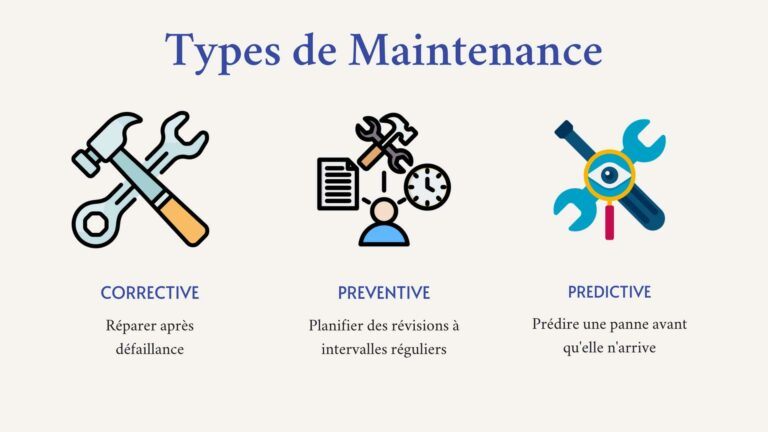
\includegraphics[width=0.85\textwidth]{images/types-de-maintenance.jpg}
\caption{Types de maintenance industrielle}
\label{fig:maintenance_evolution}
\end{figure}

\subsection{Enjeux économiques des temps d'arrêt}

Les temps d'arrêt imprévus (\textit{unplanned downtime}) constituent un enjeu économique majeur pour l'industrie manufacturière. Selon une analyse sectorielle réalisée par Siemens en 2024, basée sur une enquête auprès de 181 professionnels de la maintenance entre 2019 et 2023, les coûts horaires d'immobilisation varient considérablement selon le secteur \cite{siemens2024}\footnote{Ces données proviennent d'un rapport industriel (Siemens Senseye, 2024) et n'ont pas fait l'objet d'une validation académique indépendante par des revues évaluées par les pairs. Elles sont utilisées ici pour contextualiser l'enjeu stratégique de la maintenance prédictive.} :

\begin{itemize}
\item Biens de consommation courante (FMCG) : 36\,000\,\$/heure
\item Industrie automobile : jusqu'à 2,3\,millions\,\$/heure dans les grandes usines
\item Petites et moyennes entreprises : environ 150\,000\,\$/heure
\end{itemize}

À l'échelle macroéconomique, les pertes annuelles attribuées aux temps d'arrêt non planifiés pour les 500 plus grandes entreprises mondiales sont estimées à 1,4~trillion de dollars \cite{siemens2024}. Le potentiel d'économie associé à l'adoption de la Maintenance Prédictive (PdM) est régulièrement chiffré dans les rapports industriels à une réduction des coûts de maintenance de l'ordre de 40\,\% \cite{siemens2024}. Ces projections, si elles se confirment à grande échelle, représenteraient des économies significatives pour les entreprises industrielles.

\subsection{Défis pour les petites et moyennes entreprises (PME)}

Malgré le potentiel économique de la PdM, les solutions traditionnelles d'intelligence artificielle (IA) et d'Internet des objets (IoT, \textit{Internet of Things}) restent complexes et coûteuses à déployer, notamment pour les petites et moyennes entreprises (PME) \cite{siemens2024}. Ces dernières font face à des barrières significatives pour l'adoption de la maintenance prédictive \cite{oecd2021} :
\begin{itemize}
\item Coût prohibitif des solutions commerciales (>5\,000\,€)
\item Absence d'expertise IA/IoT interne
\item ROI incertain pour équipements auxiliaires
\end{itemize}

Le paradigme TinyML, en permettant l'implémentation de modèles ML directement sur des microcontrôleurs à faible coût, pourrait offrir une alternative plus accessible pour la détection d'anomalies vibratoires en environnements contraints.

\section{Analyse vibratoire}
\label{sec:analyse_vibratoire}

L'analyse vibratoire est la modalité de surveillance la plus courante et la plus performante pour le \textit{Condition Monitoring} des machines tournantes, car la vibration est la modalité de référence standardisée pour l'évaluation de l'état de ces équipements (ISO 20816/17359) \cite{iso20816-1,hassan2024}. Les défauts mécaniques tels que le désalignement, le balourd, les roulements endommagés ou les défauts d'engrenage génèrent des signatures distinctes dans les signaux vibratoires \cite{tiboni2022}.

\subsection{Cadre normatif et évaluation}

L'évaluation des vibrations est encadrée par les normes internationales de l'Organisation Internationale de Normalisation (ISO), notamment la série ISO 20816.

La \textbf{Norme ISO 20816-1:2016} \cite{iso20816-1} établit les lignes directrices générales pour la mesure et l'évaluation des vibrations mécaniques des machines, applicable aux mesures effectuées sur les parties tournantes (arbres) et non tournantes (paliers) en conditions de fonctionnement stable. Elle stipule que l'évaluation se fait typiquement en considérant l'amplitude de la vibration large bande observée. Elle précise également les quantités de mesure (déplacement, vitesse, accélération) et la plage de réponse en fréquence requise, qui est d'au moins 10\,Hz à 1\,000\,Hz pour l'évaluation de la vitesse efficace (r.m.s.).

La \textbf{Norme ISO 20816-3:2022} \cite{iso20816-3} est un document sectoriel qui spécifie les exigences pour l'évaluation des vibrations des machines industrielles accouplées d'une puissance nominale supérieure à 15\,kW et fonctionnant entre 120\,tr/min et 30\,000\,tr/min. Elle fournit des critères d'évaluation pour les mesures effectuées \textit{in-situ} sur des paliers ou des supports de palier.

Par ailleurs, la \textbf{Norme ISO 17359:2018} \cite{iso17359} fournit les lignes directrices pour l'établissement d'un programme de surveillance d'état (CBM), incluant la sélection des variables à mesurer et la détermination des critères d'alarme.

\subsection{Acquisition de données et capteurs}

L'acquisition des données vibratoires est généralement assurée par des accéléromètres \cite{hassan2024}. Historiquement, des capteurs piézoélectriques industriels ont été utilisés, mais la tendance pour les dispositifs IoT et TinyML est à l'intégration d'accéléromètres basés sur la technologie \textbf{MEMS} (\textit{Micro-Electro-Mechanical Systems}). Les capteurs MEMS sont privilégiés pour leur faible coût, leur petite taille et leur faible consommation d'énergie, ce qui les rend idéaux pour les systèmes embarqués contraints \cite{hassan2024,arciniegas2025}.

\subsection{Traitement du signal et extraction de caractéristiques}

Le signal vibratoire brut capturé doit subir un traitement pour en extraire des caractéristiques pertinentes pour le diagnostic. Ce processus suit typiquement une chaîne en plusieurs étapes:

\begin{enumerate}
\item \textbf{Prétraitement :} Il inclut le nettoyage des données brutes pour réduire le bruit et les artefacts \cite{bagri2024}.
\item \textbf{Traitement du Signal :} C'est la conversion du signal du domaine temporel au domaine fréquentiel ou temps-fréquence.
\item \textbf{Extraction de Caractéristiques :} Calcul d'indicateurs (statistiques, fréquentiels) qui servent d'entrées aux modèles ML/DL.
\end{enumerate}

\textbf{Analyse Temporelle :} L'analyse du domaine temporel examine directement la forme d'onde enregistrée pour en extraire des descripteurs statistiques. Le niveau d'amplitude est un bon indicateur de la condition de la machine et de la gravité du défaut. Les caractéristiques couramment utilisées incluent :
\begin{itemize}
\item \textbf{La Moyenne Quadratique (RMS -- Root Mean Square) :} Mesure robuste de l'amplitude de la vibration qui est moins sensible aux variations extrêmes et plus indicative de l'énergie totale du signal.
\item \textbf{Le Kurtosis (Aplatissement) :} Indicateur statistique de la distribution des pics. Un Kurtosis élevé peut signaler des défauts précoces dans les roulements.
\end{itemize}

\textbf{Analyse Fréquentielle (FFT) :} La Transformation de Fourier Rapide (FFT), introduite par Cooley et Tukey \cite{cooley1965}, convertit le signal temporel en spectre de fréquences pour identifier les \textbf{fréquences caractéristiques} des défauts (par exemple, balourd près de $1 \times F_r$, désalignement près de $2 \times F_r$, où $F_r$ est la fréquence de rotation). Le \textbf{théorème de Nyquist} impose une fréquence d'échantillonnage $f_s \geq 2f_{max}$ pour éviter l'aliasing. La norme ISO 20816-1 spécifie typiquement une analyse jusqu'à 1\,kHz pour les machines tournantes \cite{iso20816-1}. Les choix pratiques (fenêtrage, taille FFT, résolution) relèvent de la \textbf{méthodologie expérimentale} (chapitre suivant).

\subsection{Caractéristiques vibratoires courantes}

L'efficacité de la détection d'anomalies dépend de l'extraction de caractéristiques pertinentes. La littérature identifie deux catégories principales \cite{ran2019,tiboni2022} :

\textbf{Domaine temporel :}
\begin{itemize}
\item \textbf{RMS} : indicateur d'énergie globale du signal.
\item \textbf{Valeur crête / facteur de crête} : sensibles aux chocs localisés.
\item \textbf{Kurtosis} : met en évidence des pics marqués (défauts précoces de roulements).
\item \textbf{Skewness} : révèle des asymétries.
\end{itemize}

\textbf{Domaine fréquentiel :}
\begin{itemize}
\item \textbf{Pics harmoniques} : amplitude à $1 \times F_r$ (balourd), $2 \times F_r$ (désalignement).
\item \textbf{Bandes fréquentielles} : basses fréquences (défauts mécaniques), hautes fréquences (roulements).
\item \textbf{Enveloppe} : démodulation pour détecter signatures des roulements.
\end{itemize}


\section{Détection d'anomalies par Apprentissage Automatique}
\label{sec:detection_anomalies}

L'apprentissage automatique (ML) est au cœur de la PdM pour l'identification et la classification autonomes des schémas de comportement anormaux \cite{achouch2022,chandola2009}. Le choix de la méthode dépend crucialement de la disponibilité de données étiquetées de défaillance, souvent rares en environnement industriel.

\subsection{Approches non supervisées et semi-supervisées}

Les méthodes non supervisées sont essentielles pour la détection d'anomalies (AD) dans les scénarios industriels où la majorité des données représentent un fonctionnement normal (état sain) \cite{arciniegas2025}. Ces algorithmes modélisent le comportement normal et signalent tout écart significatif.

\textbf{K-means} \cite{macqueen1967,chandola2009} : Méthode de partitionnement non supervisée qui regroupe des observations présentant des caractéristiques proches. En maintenance, elle sert à modéliser la \textbf{normalité} et à signaler comme \textbf{anomalies} les observations très éloignées des centroïdes. Atouts : simplicité, faible empreinte mémoire, interprétabilité. Points d'attention : hypothèse de clusters compacts, choix de $k$.

\textbf{Isolation Forest (IF) :} Cet algorithme, particulièrement efficace pour l'AD, isole les anomalies en utilisant des partitions aléatoires. Il est performant et adapté à l'embarqué. Antonini et al. (2023) l'ont utilisé sur microcontrôleur, réalisant une détection d'anomalie en moins de 16\,ms avec 84\,Ko de RAM \cite{antonini2023} (voir note matérielle §1.5.3).

\textbf{Autoencodeurs (AE) :} Les autoencodeurs sont des réseaux neuronaux non supervisés entraînés à reconstruire les données d'entrée. Ils excellent à modéliser la \textit{normalité}. Une erreur de reconstruction élevée indique une anomalie \cite{ran2019}. Les AE sont utilisés pour la détection d'anomalies dans la maintenance prédictive, notamment en environnement embarqué.

\subsection{Approches supervisées et apprentissage profond}

Lorsque des \textbf{données de défauts étiquetées} sont disponibles, des classifieurs (p.~ex. SVM, forêts) et des réseaux (CNN-1D, LSTM/GRU) offrent souvent une \textbf{excellente précision} en exploitant directement les formes d'onde ou des représentations temps-fréquence \cite{bagri2024,langer2025}. En pratique, ces approches demandent \textbf{plus de ressources} et une \textbf{quantification}/optimisation soignées, ce qui motive l'usage de méthodes \textbf{non supervisées} lorsque l'étiquetage est limité \cite{ran2019}.

\begin{table}[ht]
\centering
\caption{Comparaison des méthodes d'apprentissage automatique pour la détection d'anomalies embarquée}
\label{tab:ml_comparison}
\begin{tabular}{llll}
\toprule
\textbf{Méthode} &
\textbf{Usage PdM} &
\textbf{Points clés} &
\textbf{Réf.} \\
\midrule

K-means &
Adapté &
Léger, choix de $k$ critique &
\cite{macqueen1967,chandola2009} \\

Isolation Forest &
Adapté &
Anomalies rares, réglages &
\cite{chandola2009,antonini2023} \\

One-Class SVM &
Cas spécifiques &
Frontière décision, hyperparamètres &
\cite{chandola2009} \\

Autoencodeurs &
Si optimisé &
Reconstruction, définition seuils &
\cite{chandola2009,ran2019} \\

CNN/LSTM &
Quantification requise &
Extraction automatique, ressources élevées &
\cite{langer2025,arciniegas2025} \\

\bottomrule
\end{tabular}
\end{table}


\section{TinyML Industriel}
\label{sec:tinyml_industriel}

Le TinyML est l'extension de l'intelligence artificielle jusqu'aux dispositifs d'extrémité (\textit{extreme edge}), permettant l'exécution de modèles ML directement sur des microcontrôleurs (MCU) à ultra-faible consommation \cite{tsoukas2024,njor2024}. Ce changement de paradigme est fondamental pour la PdM, car il supprime les dépendances à la connectivité réseau et réduit drastiquement la latence.

\subsection{Définition et Contraintes Techniques}

Le TinyML se déploie généralement sur des microcontrôleurs 32 bits caractérisés par des ressources matérielles extrêmement limitées. Les contraintes typiques sont sévères :
\begin{itemize}
\item \textbf{Mémoire vive (SRAM) :} de l'ordre de quelques centaines de kilo-octets.
\item \textbf{Mémoire flash (stockage) :} Habituellement limitée (quelques Mo).
\item \textbf{Consommation énergétique :} Faible, souvent de l'ordre du milliwatt.
\end{itemize}

Ces contraintes imposent l'utilisation de modèles ML extrêmement légers. L'objectif principal est de permettre une inférence en temps réel avec une latence minimale. Il est important de distinguer deux métriques :
\begin{itemize}
\item \textbf{Latence d'inférence :} quelques millisecondes à quelques dizaines de millisecondes selon l'application.
\item \textbf{Latence système totale :} souvent < 100\,ms (acquisition + prétraitement + inférence + alerte), ce qui reste compatible avec les exigences industrielles de surveillance en temps réel.
\end{itemize>

\subsection{Chaîne d'outils et Optimisation}

Les déploiements TinyML combinent un moteur d'inférence pour microcontrôleurs, un pipeline de traitement du signal (p.~ex. FFT) et des techniques d'optimisation (quantification, éventuellement \textit{pruning}) afin de réduire l'empreinte mémoire et la latence tout en préservant la détection \cite{tsoukas2024,arciniegas2025,langer2025}.

\subsection{Cas d'application en détection d'anomalies vibratoires}

Des travaux récents démontrent la \textbf{faisabilité} de la détection d'anomalies vibratoires en temps quasi réel sur microcontrôleurs, avec des approches et performances variables selon les configurations matérielles et algorithmiques :

\textbf{Antonini et al. (2023)} \cite{antonini2023} ont validé un système basé sur \textbf{Isolation Forest} sur microcontrôleur \textbf{ESP32\_WROVER\_IE} (avec mémoire externe PSRAM), démontrant une robustesse en environnements industriels extrêmes (-40°C à +85°C) avec des latences d'inférence de l'ordre de quelques dizaines de millisecondes.

\textbf{Note matérielle :} Ces résultats ont été obtenus sur une configuration disposant de mémoire externe (PSRAM); la transposabilité dépend des ressources disponibles sur le microcontrôleur cible.

D'autres études \cite{arciniegas2025,langer2025,gupta2025} rapportent des implémentations TinyML utilisant des réseaux neuronaux quantifiés (CNN-1D) pour la détection vibratoire, avec des précisions variables en laboratoire. Les performances dépendent fortement du \textbf{contexte matériel}, des \textbf{paramètres de traitement du signal} (taille FFT, fenêtrage) et des \textbf{compromis mémoire/latence} adoptés.

Le TinyML permet théoriquement le déport d'une capacité analytique sophistiquée (y compris \textit{Deep Learning} ou algorithmes d'ensemble) directement sur des dispositifs peu coûteux et autonomes, visant une détection d'anomalies à faible latence potentiellement compatible avec les exigences industrielles en temps réel.

Il est important de reconnaître que la majorité des travaux académiques sur le TinyML pour la maintenance s'appuient sur des validations en laboratoire avec des défauts contrôlés. Cette approche méthodologique, bien que nécessaire pour établir la faisabilité technique, constitue une première étape vers le déploiement industriel. Les défis de la maintenance à long terme et l'adaptation aux conditions industrielles variables restent des axes de recherche ouverts pour l'ensemble de la communauté scientifique. Les compromis entre latence, précision et ressources varient selon les chaînes de traitement et nécessitent des validations spécifiques.

\section{Synthèse critique et positionnement}
\label{sec:synthese_critique}

L'analyse de l'état de l'art confirme que la Maintenance Prédictive (PdM) est un impératif économique pour l'industrie, essentiel pour contrecarrer les coûts prohibitifs des arrêts non planifiés (variant de 36\,000\,\$/heure à 2,3 millions\,\$/heure selon le secteur \cite{siemens2024}). La surveillance vibratoire, encadrée par les normes ISO 20816, est la méthode de prédilection, avec une complexité d'analyse gérable grâce à l'extraction de caractéristiques fréquentielles (FFT).

Le paradigme TinyML offre une opportunité prometteuse pour explorer des approches d'IA plus accessibles pour les systèmes de surveillance contraints. Les études de cas récentes (Antonini 2023, Arciniegas 2025, Langer 2025) ont démontré la faisabilité technique de la détection d'anomalies en temps réel (<100\,ms) en utilisant des microcontrôleurs et des modèles optimisés \cite{antonini2023,arciniegas2025,langer2025}.

Cependant, plusieurs lacunes persistent dans la littérature :

\begin{itemize}
\item \textbf{Rareté des données de défauts :} l'étiquetage limité favorise les méthodes non supervisées et complique les comparaisons.
\item \textbf{Benchmarks vibration-TinyML :} peu de références \textbf{standardisées}, comparabilité difficile \cite{banbury2021}.
\item \textbf{Portabilité des résultats :} performances très dépendantes des \textbf{ressources} et du \textbf{traitement du signal}; validations souvent en \textbf{laboratoire} \cite{antonini2023,arciniegas2025,langer2025}.
\end{itemize}

\textbf{Positionnement critique :} L'analyse de l'état de l'art révèle un décalage entre le potentiel économique théorique de la PdM (économies projetées de 40\,\% des coûts de maintenance selon les rapports industriels \cite{siemens2024}) et les défis pratiques du déploiement TinyML sur microcontrôleurs contraints. Les contraintes matérielles (mémoire limitée, puissance de calcul réduite) imposent des compromis algorithmiques qui peuvent affecter la précision de détection. De plus, la majorité des validations expérimentales publiées s'appuient sur des conditions de laboratoire avec des défauts contrôlés \cite{antonini2023,arciniegas2025,langer2025}, laissant ouverte la question de la robustesse en environnement industriel réel avec variabilité des charges, conditions environnementales, et modes de dégradation progressifs.

Ces lacunes identifiées orientent vers le développement de solutions adaptées aux contraintes industrielles réelles, dont la conception sera détaillée dans le chapitre suivant.

%%%%%%%%%%%%%%%%%%%%%%%%%%%%%%%%%%%%%%%%%%%%%%%%%%%%%%%%%%%
% BIBLIOGRAPHIE
%%%%%%%%%%%%%%%%%%%%%%%%%%%%%%%%%%%%%%%%%%%%%%%%%%%%%%%%%%%
\cleardoublepage
\renewcommand{\bibname}{Bibliographie}
\bibliographystyle{IEEEtran}
\bibliography{bibliographie}

\end{document}